%! Author = dmitriy
%! Date = 9/15/23

% Preamble
\documentclass[14pt]{extreport}
\usepackage{gost}
\usepackage{ragged2e}
%\usepackage{blindtext}
\justifying
\renewcommand{\thefigure}{\arabic{figure}}
\renewcommand{\thetable}{\arabic{table}}

\begin{document}
    \pagestyle{empty}
    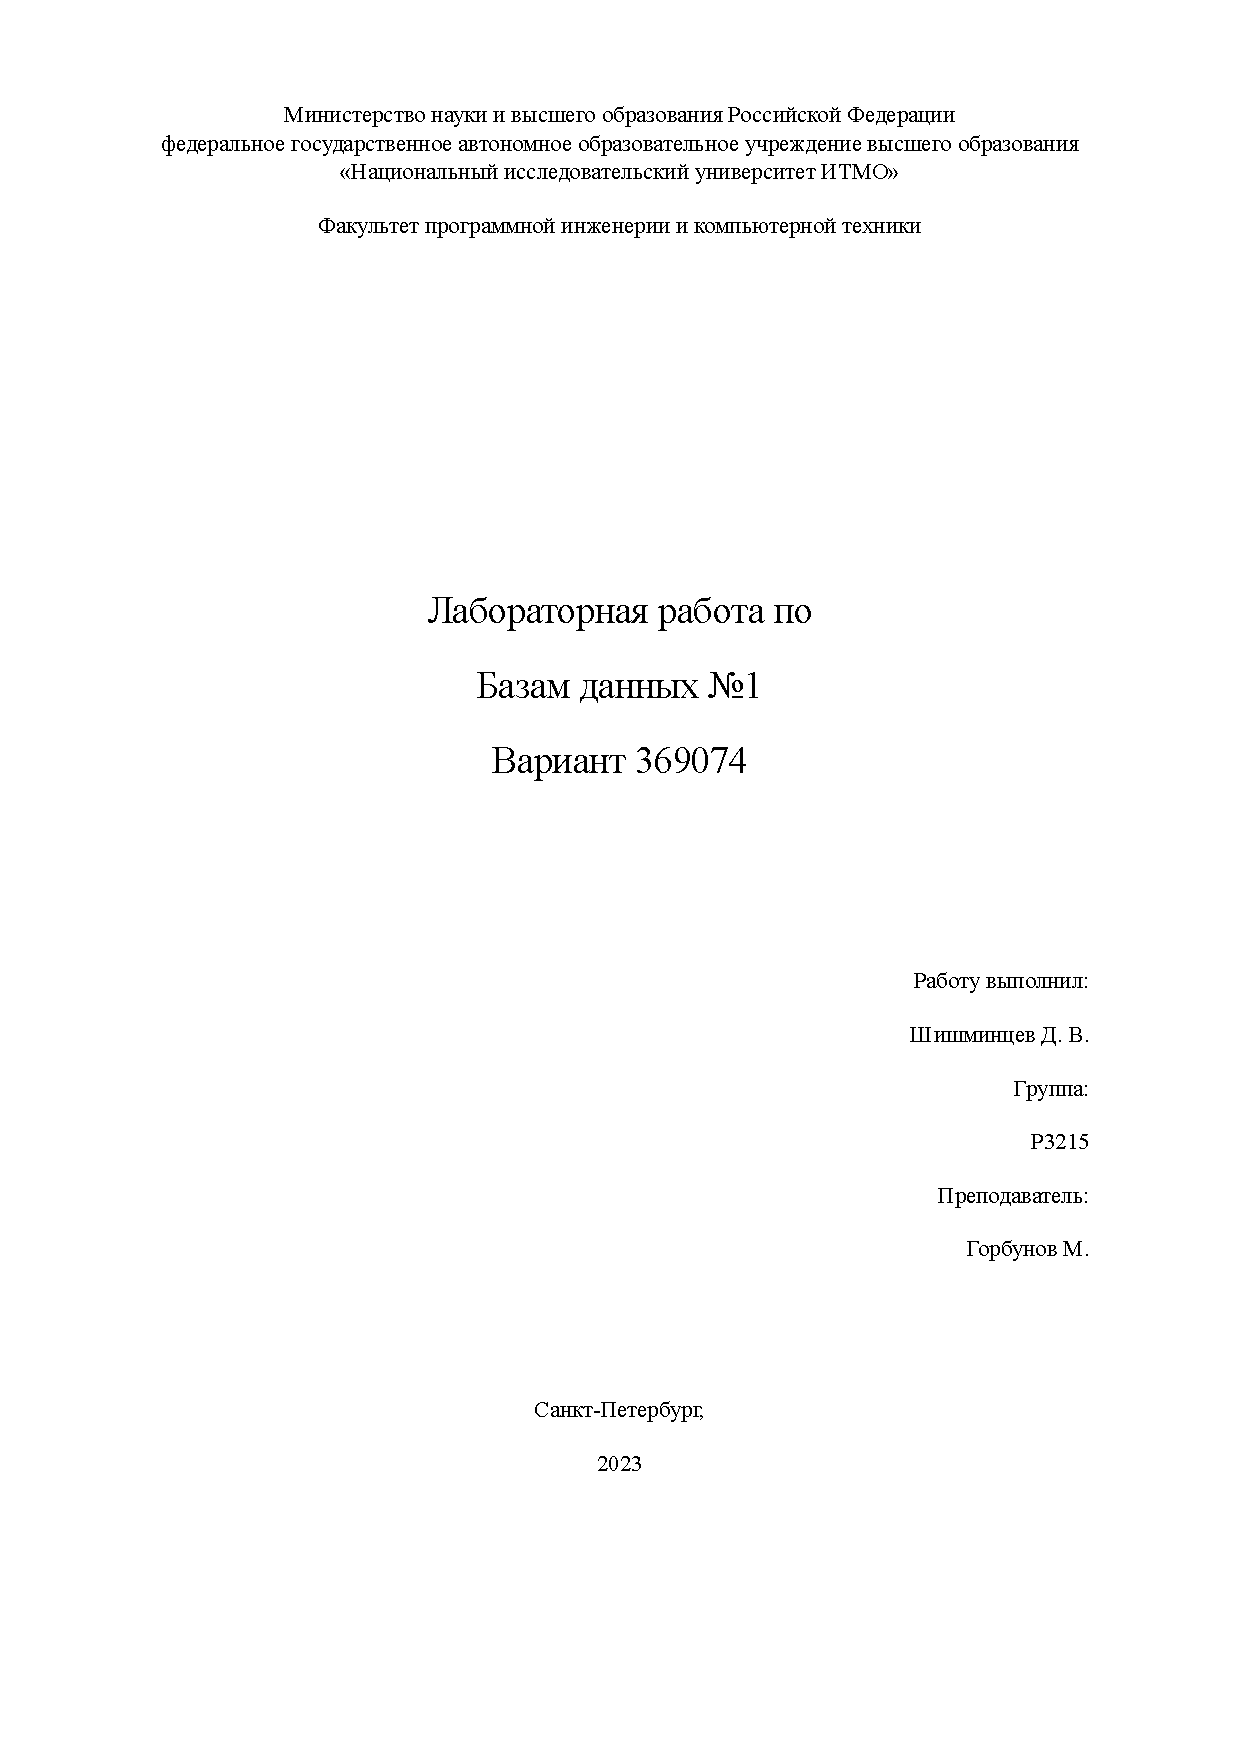
\includepdf[pages=-,pagecommand={}]{title.pdf}
    \pagestyle{plain}
    \tableofcontents

    \intro Целью данной лабораторной работы является создание базы данных на основе предложенной предметной области. В процессе выполнения работы мы будем составлять инфологическую и даталогическую модели, учитывая типы данных, характерные для СУБД PostgreSQL. Кроме того, мы реализуем даталогическую модель в PostgreSQL, обеспечивая соблюдение ограничений целостности. Завершающим этапом работы будет заполнение созданных таблиц тестовыми данными.

    \chapter{Предметная область}
    \section{Текст задания}
            Ян Малкольм лежал на спине, кожа у него была бледно-серого цвета, рот широко открыт. Дыхание вырывалось изо рта с жуткими хрипами. Малдун протянул Дженнаро фонарь и наклонился, осматривая пострадавшего.

    \section{Сущности и их атрибуты}
        \subsection{Стержневые сущности}
            Пациент:
            \begin{itemize}
                \item patient\_id - Уникальный идентификатор пациента
                \item name - Имя пациента
                \item position - Положение пациента
                \item skin\_color - Цвет кожи пациента
                \item condition - Состояние пациента
            \end{itemize}
                \bigskip


            Медицинские работники:
            \begin{itemize}
                \item staff\_id - Уникальный идентификатор медицинского работника
                \item name - Имя медицинского работника
                \item role - Роль работника
            \end{itemize}

        \subsection{Характиристические сущности}
            Инструменты:
            \begin{itemize}
                \item instrument\_id - Уникальный идентификатор инструмента
                \item name - Название
            \end{itemize}
            \bigskip


        Осмотры:
        \begin{itemize}
            \item examindation\_id - Уникальный идентификатор осмотра
            \item patient\_id - Идентификатор пациента
            \item staff\_id - Идентификатор мед. работника.
            \item examination\_time - Время проведения осмотра
        \end{itemize}
    \bigskip


    Передача инструментов:
    \begin{itemize}
        \item transfer\_id - Уникальный идентификатор инструмента
        \item from\_staff\_id - Кто передал
        \item to\_staff\_id - Кому передал
        \item instrument\_id - Идентификатор инструмента
        \item transfer\_time - Время передачи
    \end{itemize}


    \chapter{Модели}
    \section{Инфологическая модель}
            \begin{figure}[h]
                \centering
                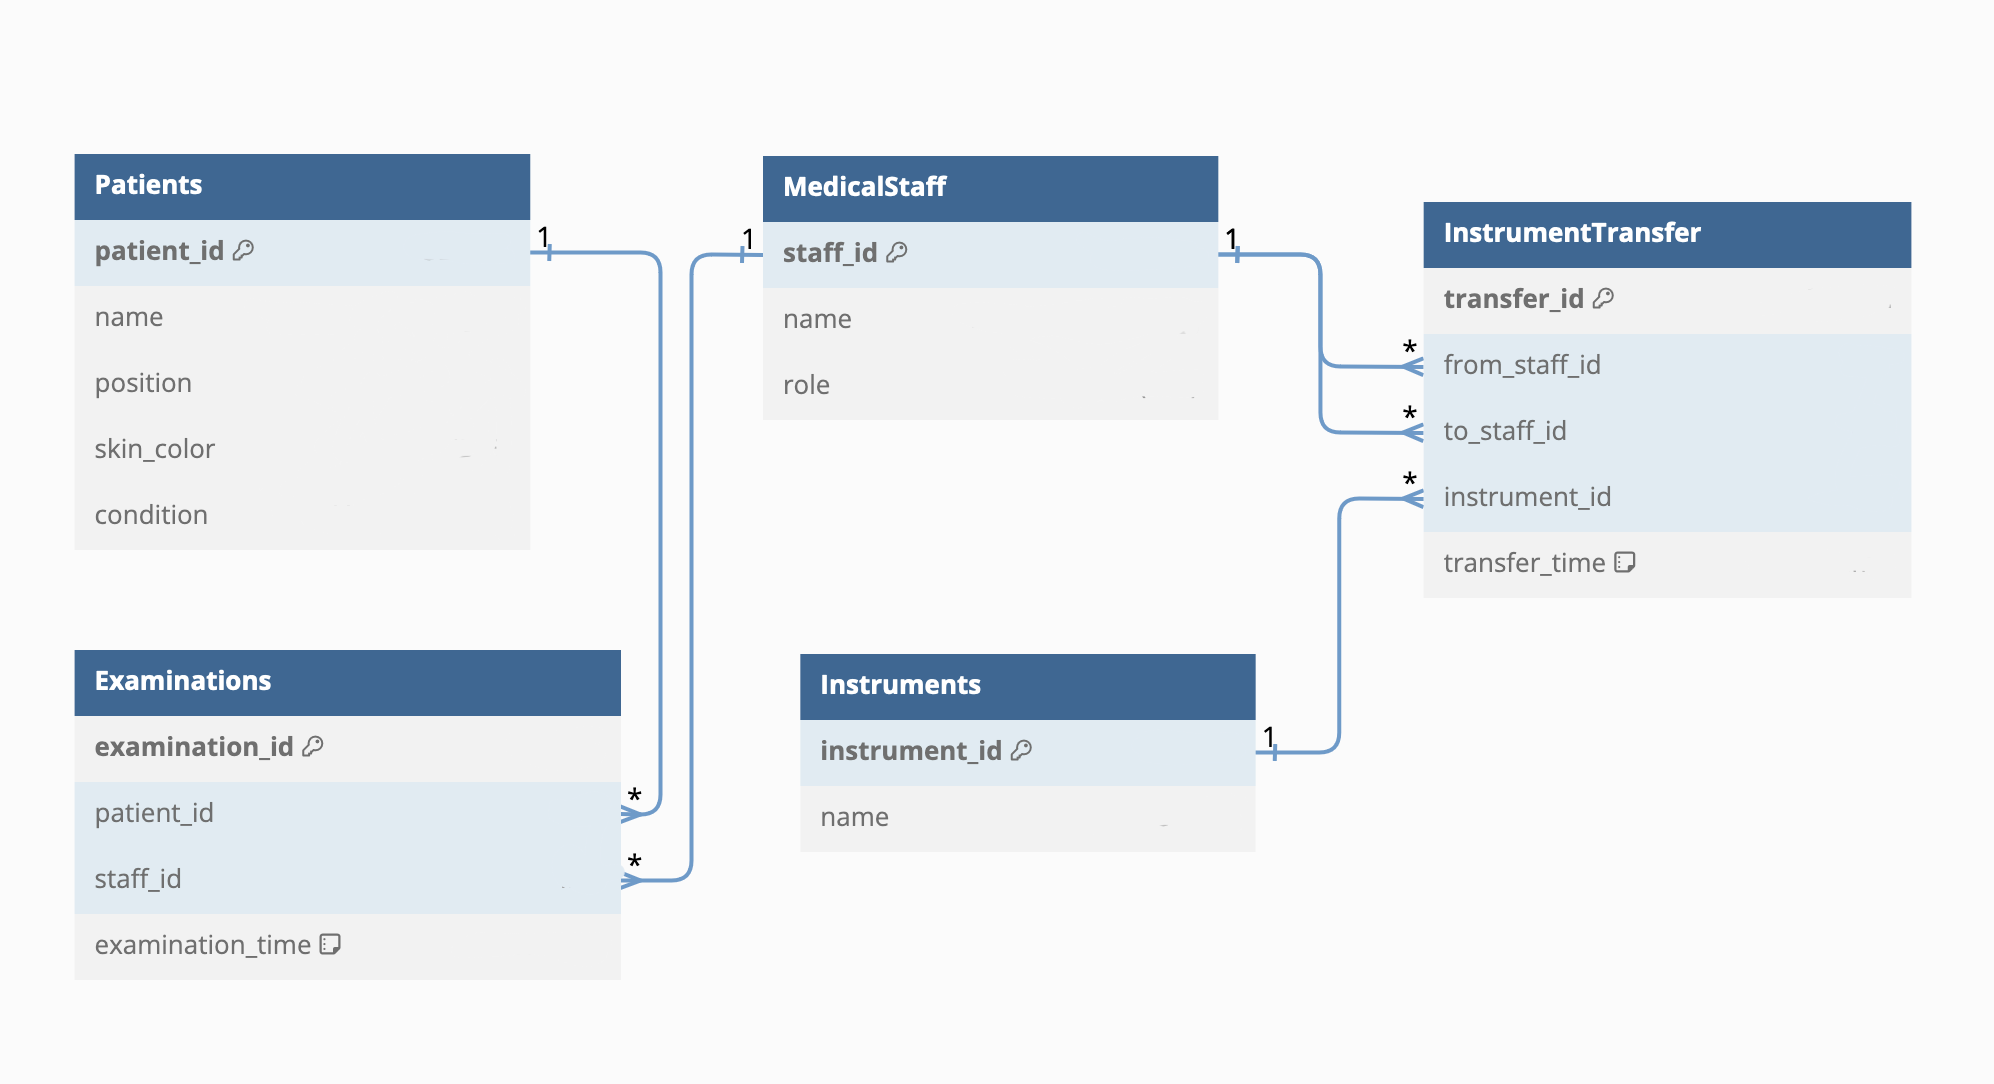
\includegraphics[width=0.75\linewidth]{er.png}
                \caption{ ER-диаграмма}
                \label{fig:d1}
            \end{figure}
    \section{Даталогическая модель}
            \begin{figure}[h]
                \centering
                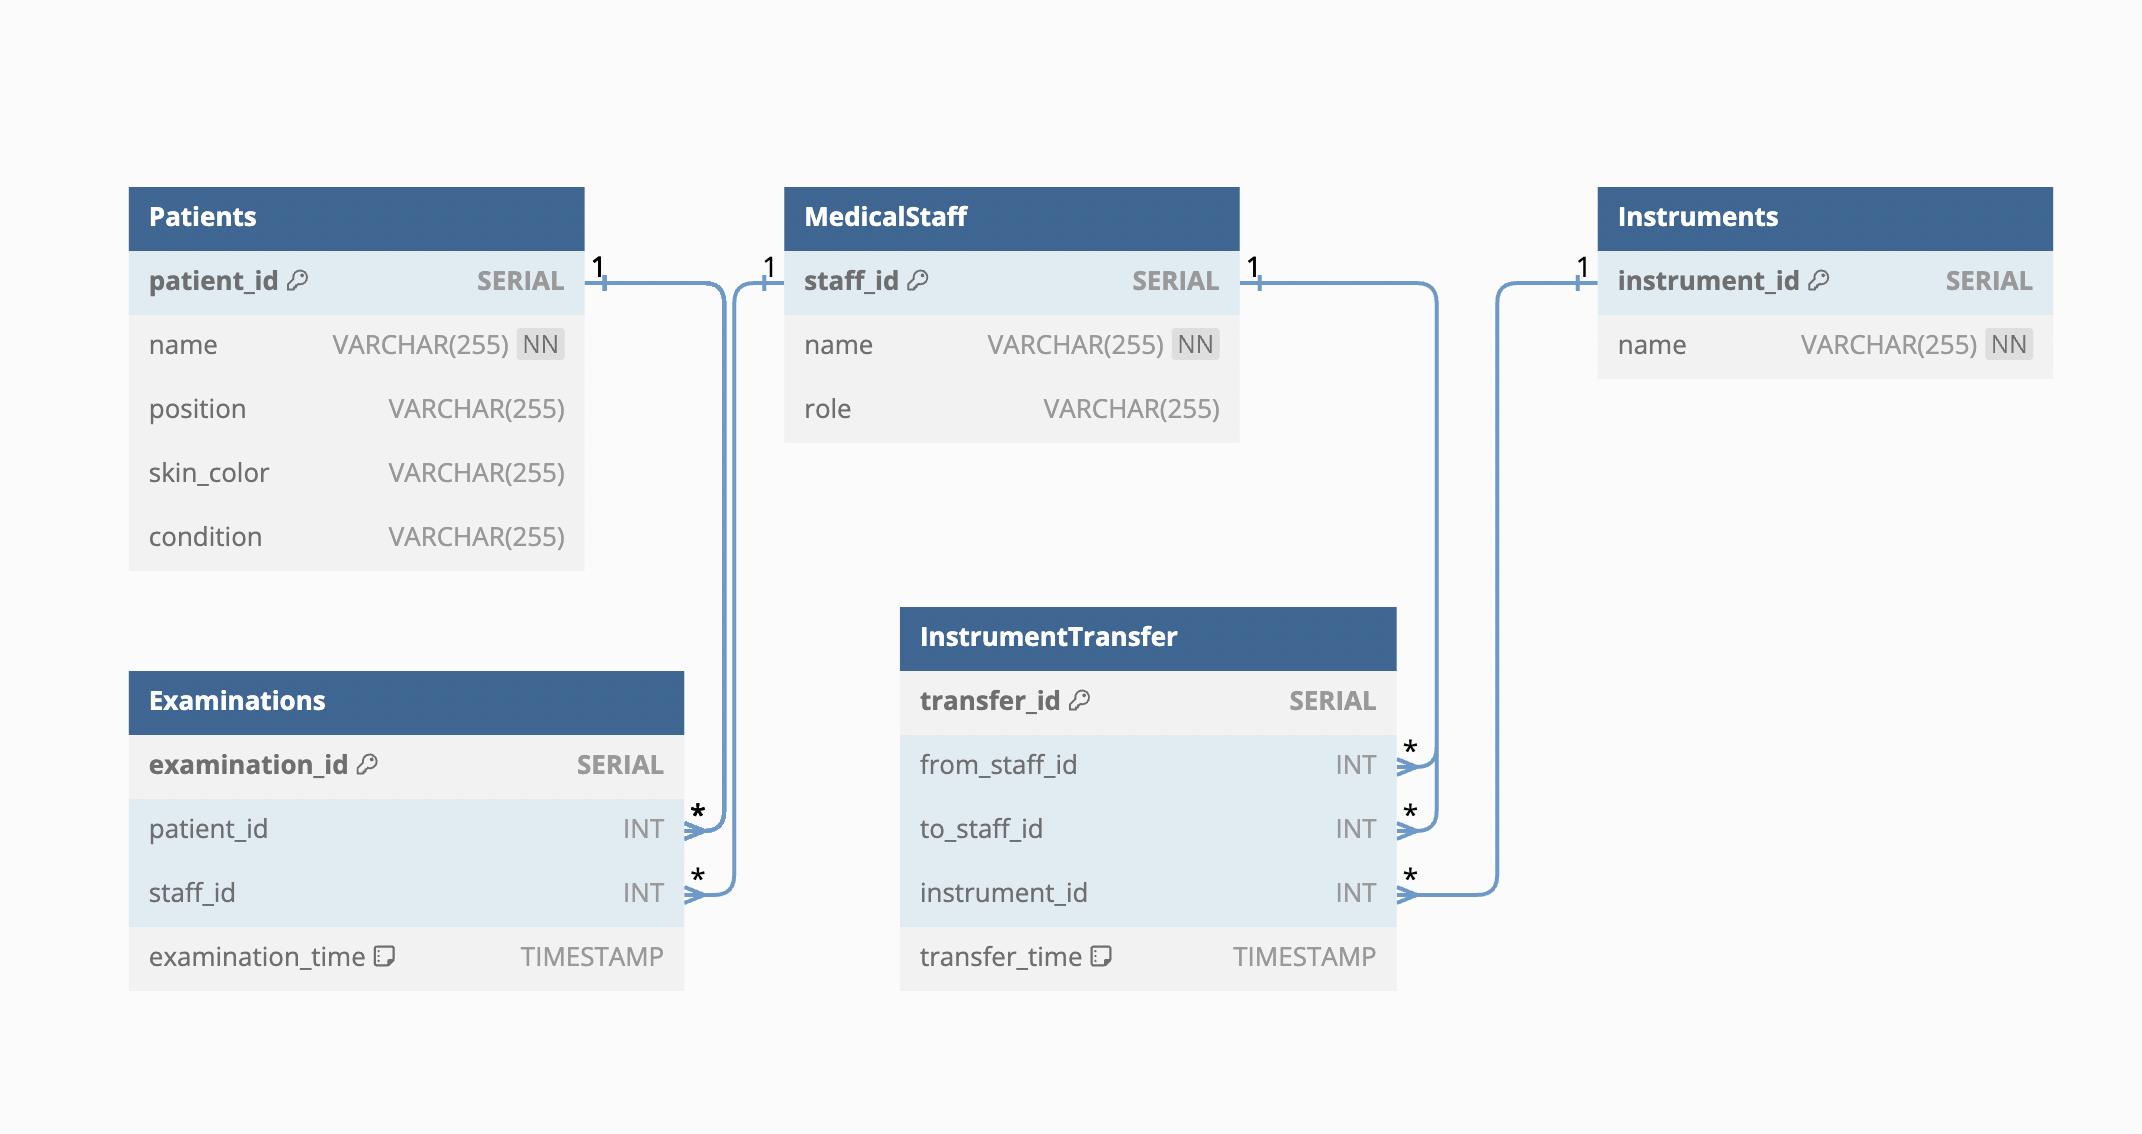
\includegraphics[width=0.75\linewidth]{ddl.png}
                \caption{ Датологическая модель}
                \label{fig:d2}
            \end{figure}
\newpage
    \section{Реализация датологической модели на SQL}
    \begin{verbatim}
CREATE TABLE Patients (
    patient_id SERIAL PRIMARY KEY,
    name VARCHAR(255) NOT NULL,
    position VARCHAR(255),
    skin_color VARCHAR(255),
    condition VARCHAR(255)
);
CREATE TABLE MedicalStaff (
    staff_id SERIAL PRIMARY KEY,
    name VARCHAR(255) NOT NULL,
    role VARCHAR(255)
);
CREATE TABLE Instruments (
    instrument_id SERIAL PRIMARY KEY,
    name VARCHAR(255) NOT NULL
);
CREATE TABLE InstrumentTransfer (
    transfer_id SERIAL PRIMARY KEY,
    from_staff_id INT REFERENCES MedicalStaff(staff_id),
    to_staff_id INT REFERENCES MedicalStaff(staff_id),
    instrument_id INT REFERENCES Instruments(instrument_id),
    transfer_time TIMESTAMP DEFAULT CURRENT_TIMESTAMP
);
CREATE TABLE Examinations (
    examination_id SERIAL PRIMARY KEY,
    patient_id INT REFERENCES Patients(patient_id),
    staff_id INT REFERENCES MedicalStaff(staff_id),
    examination_time TIMESTAMP DEFAULT CURRENT_TIMESTAMP
);
    \end{verbatim}


    \conclusions В результате выполнения лабораторной работы была разработана база данных, которая отражает предметную область с учетом сущностей, атрибутов и связей. Мы создали инфологическую и даталогическую модели, а также успешно реализовали даталогическую модель в PostgreSQL.
\end{document}